%% Thesis
\documentclass[11pt,a4paper]{article}
\usepackage[top=2.5cm, bottom=2cm, left=2cm, right=2cm]{geometry}
\usepackage{amsmath}
\usepackage{mathtools}
\usepackage{gensymb}
\usepackage{tikz}
\usepackage{circuitikz}
\usepackage{epigraph}
\usepackage{hyperref}
\usepackage{multirow}
%\usepackage[demo]{graphicx}
\usepackage{caption}
\usepackage{subcaption}
\setcounter{secnumdepth}{5}
\usepackage{chngcntr}
\counterwithin{figure}{section}
\counterwithin{table}{section}
\usepackage{multirow}
\setcounter{tocdepth}{5}
\usepackage{subfiles}
\usepackage{epstopdf}
\usepackage[section]{placeins}
%\usepackage{undertilde}

% pseudocode
\usepackage{algorithm}
\usepackage[noend]{algpseudocode}


\renewcommand\epigraphflush{flushright}
\renewcommand\epigraphsize{\normalsize}
\setlength\epigraphwidth{0.7\textwidth}

\usepackage[]{color}
\definecolor{titlepagecolor}{cmyk}{1,.0,0.0,.50}
\definecolor{scolour}{cmyk}{1,.0,0.0,.85}
\definecolor{sscolour}{cmyk}{1,.0,0.0,.75}
\definecolor{ssscolour}{cmyk}{1,.0,0.0,.65}
\definecolor{paracolour}{cmyk}{1,.0,0.0,.55}

\usepackage{amsfonts}
%\DeclareFixedFont{\titlefont}{T1}{ams}{b}{sc}{0.5in}

% Added 
\usepackage{fancyhdr}
\pagestyle{fancy}
\lhead{Augmented Space}
\rhead{Lydia Drabsch}
\cfoot{\thepage}
\renewcommand{\headrulewidth}{0.4pt}
\renewcommand{\footrulewidth}{0.4pt}
\renewcommand{\thepage}{\roman{page}}
\usepackage{indentfirst}           %remove if we dont want to indent
\renewcommand{\thepage}{\roman{page}}
\usepackage{bibentry}

\newcommand{\myparagraph}[1]{\paragraph{#1}\mbox{}\newline\indent}
% vectors
\newcommand{\dv}[1]{\textbf{\textit{#1}}}
\newcommand{\vv}[1]{\dot{\textbf{\textit{#1}}}}
\newcommand{\av}[1]{\ddot{\textbf{\textit{#1}}}}
\renewcommand{\vec}[1]{\textbf{#1}}
\newcommand{\nvec}[1]{\hat{\textbf{#1}}}

\newlength{\normalparindent}
\AtBeginDocument{\setlength{\normalparindent}{\parindent}}

% Change heading colours
\usepackage{titlesec}
%\usepackage[usenames,dvipsnames]{xcolor}
\usepackage{bold-extra}
\titleformat{\section}
{\color{scolour}\scshape\LARGE\bfseries}
{\color{scolour}\thesection.}{2em}{}
\titleformat{\subsection}
{\color{sscolour}\normalfont\Large\bfseries}
{\color{sscolour}\thesubsection}{2em}{}
\titleformat{\subsubsection}
{\color{ssscolour}\normalfont\large\bfseries}
{\hspace*{\normalparindent}\color{ssscolour}\thesubsubsection}{1em}{}
\titleformat{\paragraph}
{\color{paracolour}\normalfont\large\bfseries}
{\hspace*{\normalparindent}\color{paracolour}\theparagraph}{1em}{}

% end added
\makeatletter                       
\def\printauthor{%                  
    {\large \@author}}              
\makeatother
\author{%
    Stefan Williams \\
    University of Sydney \\
    }

% Title image
\newcommand\titlepagedecoration{%
\tikz[remember picture,overlay] \node[opacity=1,inner sep=0pt] at ([xshift=5cm]current page.west){
\includegraphics[height=\paperheight]{./IMAGEtitle2f}};
}

% Matlab Code
\usepackage[framed]{mcode}
\newcommand{\Deg}{$^{\circ}$ }


\begin{document}
\newgeometry{top=3.7cm, bottom=4cm, left=3cm, right=3cm}
% \nobibliography*
\begin{titlepage}
% TURN OFF FOR SPEED
\titlepagedecoration

\flushright
\huge{\scshape Thesis}\\ Lydia Drabsch \\ 28th October 2017


\null\vfill
%\vspace{2cm}
\begin{minipage}{0.8\textwidth}
\centering
\rule{1\textwidth}{0.02pt}\\
\Huge{\textbf{\scshape Instantaneous Relative Positioning of Multiple GNSS Receivers}\\\rule{1\textwidth}{0.02pt}}
\\ 
\end{minipage}
%High Accuracy Instantaneous Relative Positioning of multiple GNSS Receivers

\null\vfill
\vspace*{1cm}
\noindent
\hfill
\begin{minipage}{0.45\linewidth}
    \begin{flushright}
        \printauthor
    \end{flushright}
\end{minipage}
%
\begin{minipage}{0.02\linewidth}
    \rule{1pt}{190pt}
\end{minipage}


\end{titlepage}
\newgeometry{top=2.5cm, bottom=2cm, left=2cm, right=2cm}

% \begin{figure*}[h!]
% \centering
% 
\includegraphics[width=0.99\linewidth]{./Plag}
% \label{fig:Plag}
% \end{figure*}

\setcounter{section}{0}

\tableofcontents
\listoffigures
\listoftables
\newpage
\pagenumbering{arabic}
%\renewcommand{\thepage}{\arabic{page}}
%%%%%%%%%%%%%%%%%%%%%%%%%%%%%%%%%%%%%%%%%%%%%%%%%%%%%%%%%%
\section{Abstract}


\section{Introduction}
epoch synchrosation followed by two fold optimisation process\\
need instantanous relative positioning with minimal calibration or setup of external hardware

Instantaneous Relative displacement/position between GNSS receivers.
Simulation case studies are presented to validate the mathematical models.


\section{Literature Review}

\subsection{Position Requirements}
- how/why to use position for applications\\
- absolute vs relative\\
- why use relative positioning\\
- knowing where you are positioned is important for data gathering, motion detecting and tracking, path planning\\
- formation flying, drones\\
\subsection{Relative Positioning Technology}
- line of sight methods\\
- pre-setup requirements\\
- long calibration setup?\\


- last one being GNSS
\subsection{GNSS Operational Components}
\subsubsection{Space Segment}
- current GNSS: explain GPS, GLONASS, galelao, chinese one constellations and how it works
- what orbits are they in: altitude
\subsubsection{User Segment}
- typical accuracy for civilian accessable gps\\
- military has more precise stuff\\
- lower cost receivers have only one frequency band, error in timing\\
Unfortunately, low cost GNSS receivers rarely provide official access to the GNSS raw data. Previous studies have used customised bluetooth headsets or customised android platform mobile phones to investigate algorithms on low-cost GNSS receivers. More expensive receivers do allow raw data to be utilised, however they also provide other mechanisms such as duel frequencies and more accurate clocks, rendering the new algorithm *obtuse*. The mindset of *crowd-sourcing*/customising/flexible technology is changing the way manufactures build GNSS receivers. The new Android OS platform Nougat 7.0 provides the developer raw GNSS data at the software level.  

\subsubsection{Control Segment}


\subsection{GNSS Satellite Signals}
- civilian GNSS using duel frequency, send CDMA, how decryption works\\
- what is psudorange?\\
- what is carrier phase\\
- clock bias\\






\subsection{The GNSS concept}
The base concept behind identifying the position of something using GNSS is remarkably simple. Satellite W sends out a radio signal at time X and it's position Y which the user received at time Z. The time difference is used to calculate the distance from the satellite's position. With this information from multiple satellites, the position of the user is triangulated. 


- timing comparison between satellite and receiver to find psudeorange
- ECEF frame of reference
\subsubsection{2D case}
\subsubsection{3D case}
- NLLS solve spheres
- need 4 satellites minimum
- 


\subsection{GNSS Error Sources}
- how large
\subsubsection{Clock Errors}
- timing of received signal because of low cost clock on receiver. 
\subsubsection{Receiver Noise}
- antenna phase
\subsubsection{Ephemeris Errors}
- satellite position is approximated\\
- due to gravity effects of other gravitational sources/ non-spherical earth/ what model is used?\\
- how long is the ephemeris data accurate for?\\
- actual location of satellite, where it thinks it is is based on a prediction model so its not 100\% correct. what uncertainty in this location therefore vector is there?

\subsubsection{Atmospheric Effects}
- ionosphere and troposphere refraction - speed of propagation changes which alters the time of flight
\subsubsection{Mutlipath Interference}


\subsubsection{Sagnac Effect}

\subsubsection{GNSS Error Summary}


\subsection{Multiple Receivers}
- problems arising with multiple receivers
- 

\subsection{Current GNSS algorithms}
- just reference implementation papers?
- algorithms to make it more accurate\\
- use for motion tracking\\
- performance vs cost trade off\\
(http://ieeexplore.ieee.org.ezproxy1.library.usyd.edu.au/document/7530542/)
\subsubsection{Standard Positioning Service}
- single frequency and multi frequency to remove atmospheric affects
\subsubsection{Differential GPS}
- explain what it is\\
- what setup is required \\
- abs vs rel \\
- degree of accuracy
\subsubsection{WAAS DGPS}

\subsubsection{SBAS  ?}

\subsubsection{Real Time Kinematic}

\subsubsection{Post Processing Algorithm}

\subsubsection{Single Frequency Precise Point Positioning (SF-PPP)}
Rademakers \textcolor{red}{how to say reference?} at University of Delft in the Netherlands developed a solution for finding the absolute position in open areas to a horizontal accuracy of 0.5 m. It uses a single frequency, single antenna low cost GPS receiver by connecting to the internet and using real time information to model all errors. The errors they corrected with the potential improvements are outlined in Table \ref{Table:SFPPP error table}. 
\begin{table}
\centering
\caption{Error Components and Potential Improvements for SF-PPP}
\label{Table:SFPPP error table}
\begin{tabular}{|l|l|}
\hline
\textbf{Error component} &\textbf{ Potential Improvement} \\\hline
 Ionosphere: Klobuchar model & 7 m \\\hline
 Troposphere: Saastamoinen model & 2.5 m \\\hline
Ephemeris data &  1 m \\\hline
 Satellite clock drift & 1.5 m \\\hline
 Differential code bias & 50 cm \\\hline
 Phase windup: rotation of the antenna & dm \\\hline
 Sagnac effect & 30 m \\\hline
 ROA: satellite orbit correction & up to 10 cm \\\hline
 Relativistic clock correction & up to 21 m \\\hline
 Moon-Earth interaction & 5cm (Hor) and 30 cm (Ver)\\\hline
\end{tabular}
\end{table}


\subsubsection{Duel Epoch Duel Differencing}
- Paper: High-Accuracy Differential Tracking of Low-Cost GPS Receivers\\
- have this one last as it is the most similar\\
- uses multiple receivers\\
- needs instantaneous relative distance for first point, to speed up processing and make the first few time steps more accurate, also when locking onto new satellites


\subsubsection{Summary of Algorithms ?}

% types of algorithms making gps more accurate: table with columns = types of analysis, rows= types of algorithms
- dynamic tracking (need temporal measurements) vs static measurement - no temporal\\
- post processing vs pre-processing vs realtime\\
- ground structure vs free standing\\
- absolute vs relative\\
- accuracy (how much)\\
- computation time/space required\\
- what error is each method removing\\
- what piece of data it needs (if raw)\\
- calibration required\\
- robustness -> if a satellite goes out of view does it need to re-calibrate? passing information between receivers-> is one a reference? single point of failure



\subsection{Proposed Planar Intersection Algorithm}
This new algorithm is derived from taking the difference in pseudorange between multiple receivers from one satellite and expressing the distances as planes.
\begin{figure}[h]
\centering
\caption{2D representation}
\label{fig:overall_singleS_multiR}
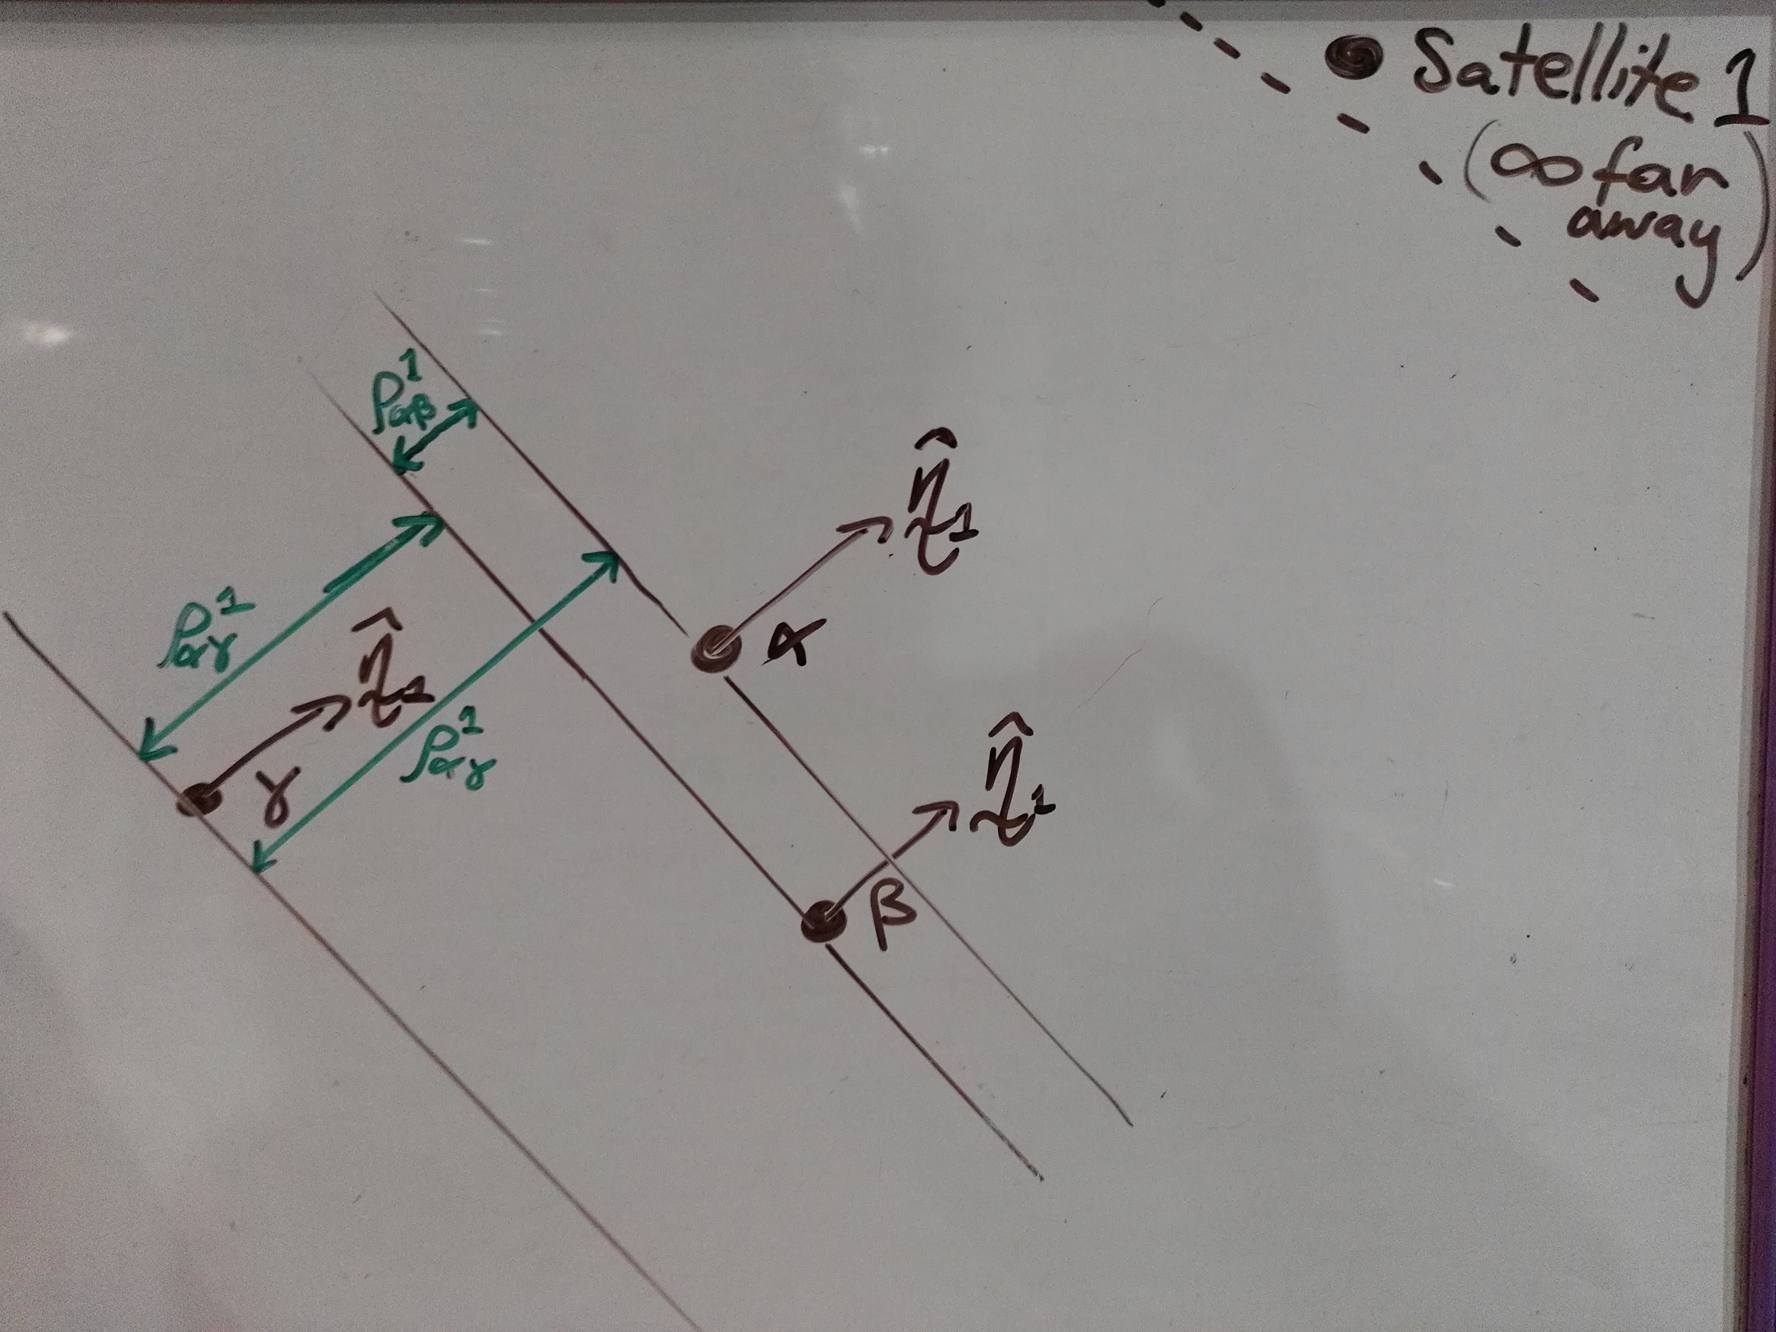
\includegraphics[width=0.7\linewidth]{overall_singleS_multiR}
\end{figure}

With multiple satellites in view, the intersection of planes for a particular receiver is the position of the receiver.
\begin{figure}[h]
\centering
\caption{}
\label{fig:overall_multiS_duelR}
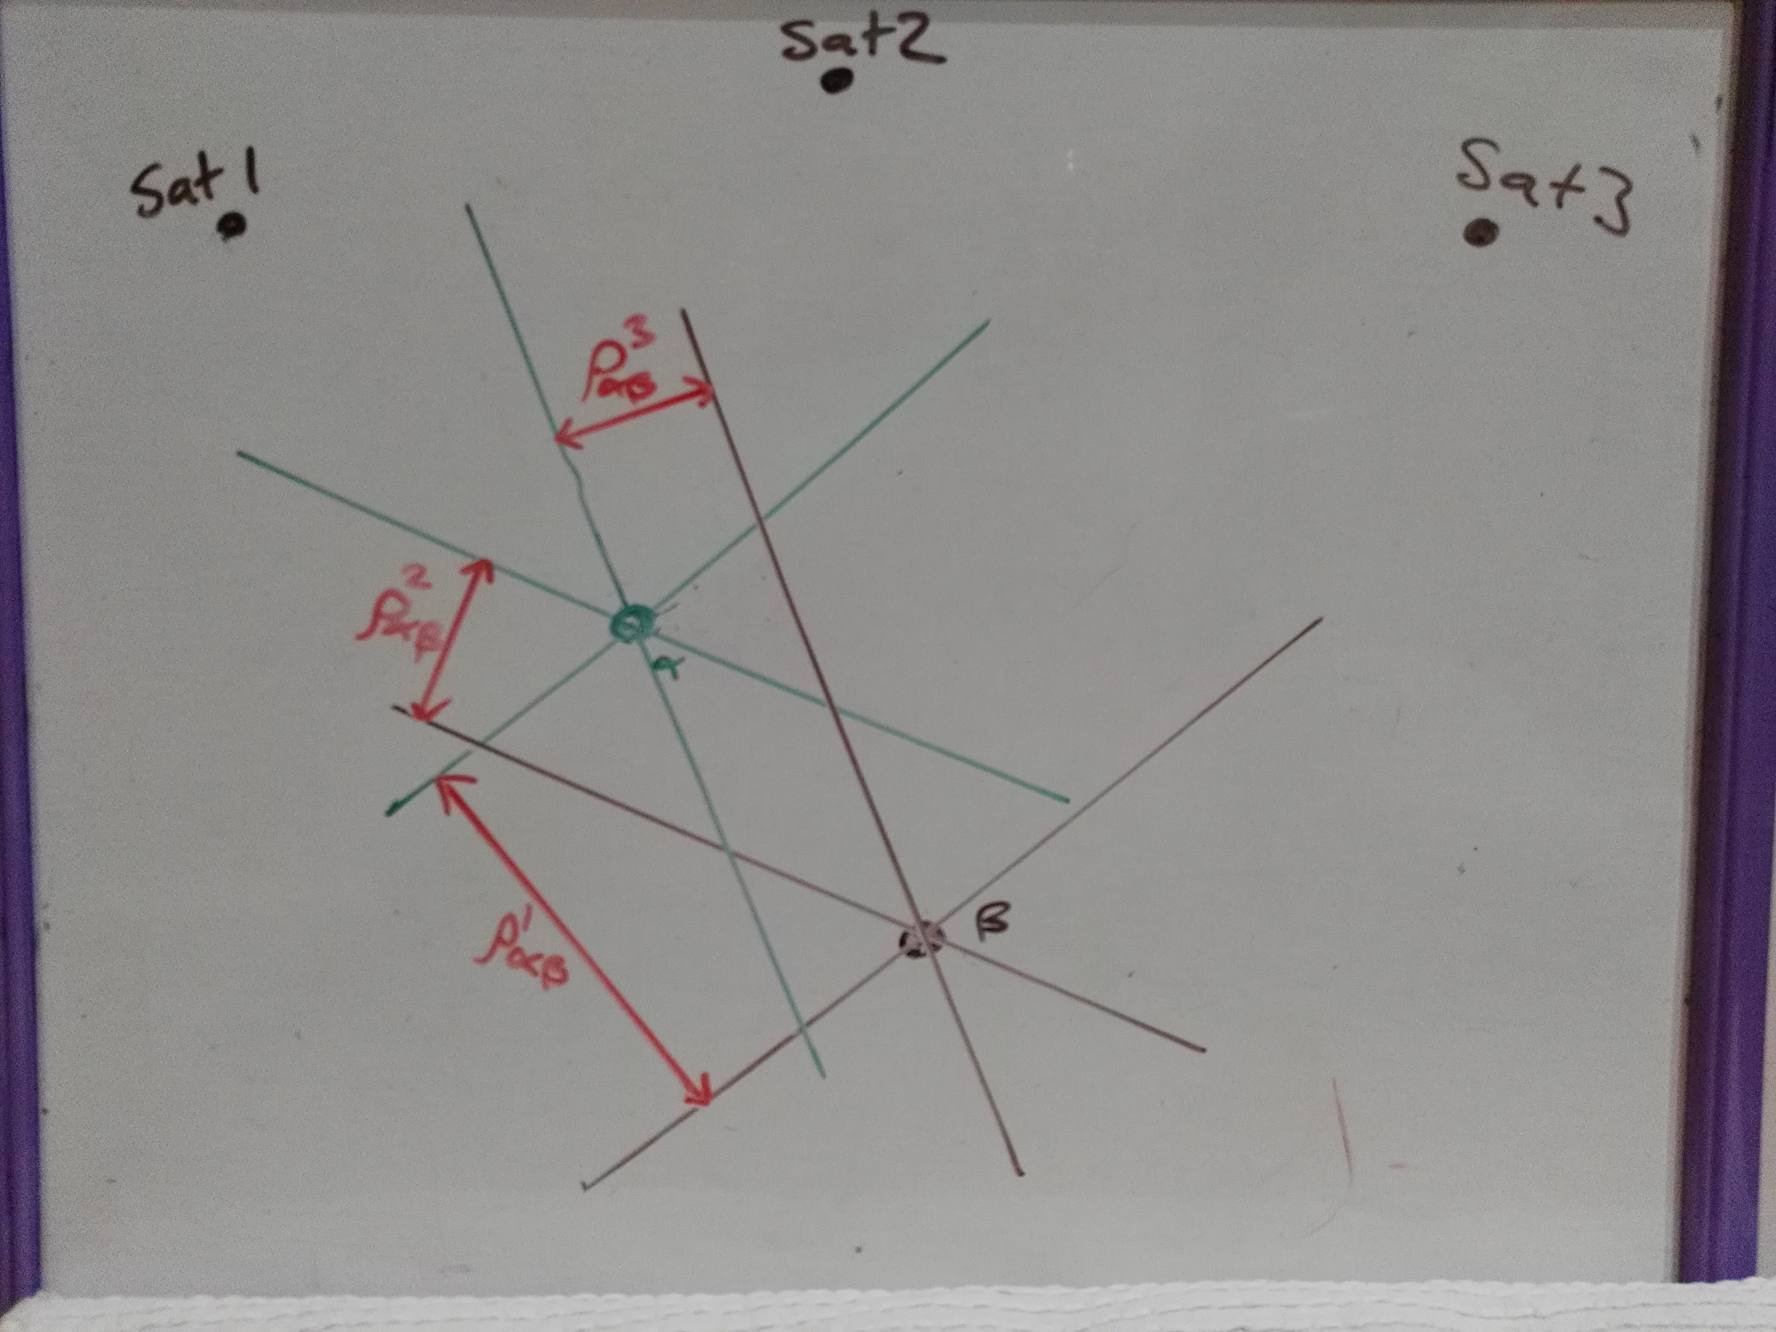
\includegraphics[width=0.7\linewidth]{overall_multiS_duelR}
\end{figure}

With this strategy, some of the errors that plague the absolute position are negated for the relative position. These include the ionospheric and tropospheric affects.









% small






%??Topical organisation with inverted pyramid substructure
% \subsubsection{GNSS Localisation}
% Global Navigation Satellite System (GNSS) 
% - lower update rates $\approx$1Hz\\
% - accuracy/precision? not good enough for these applications\\
% - not good for indoor environments as signals are weak\\
% - used differentiated gnss to solve for integer ambiguity across multiple mobile platforms on the go \cite{GNSS_difftrack} \cite{GNSS_intamb}\\
% - multipath/atmospheric error estimation \\
% - multiple receivers across the multiplayers \cite{GNSS_multi} \\

% 	%% types of precision gnss locations 
% - double differentiating - requires same satellites
% - pvt position velocity and precise time

\section{Planar Intersection Algorithm}

- assume satellite is at infinity for comparing difference in pseudorange for a particular reference satellite.\\
- use all satellites as reference satellite - no single point of failure, also not all satellites might be in view for all receivers\\
- get the normal vector between all receivers and each sat. \\
- Calculate the average normal vector.\\
- get the difference in pseudorange between all receivers along each normal vector \\
- create a plane with the normal vector with that distance\\
- solve via optimization (least squares) \\
- use clock adjustment from abs gps? or have as another optimisation variable\\
- antenna problems? misalignment?\\
- share clock bias's between solving for different reference sets? - do it one by one or all together?\\
- need to align the time of signal sent to the receivers before calculating average normal vector\\

- have weighted planes based on ? have weighted area on the planes?\\
- if one plane intercepts far away from the others then ignore it (multipath). hyperdimensional surface to minimise




% conceptual
how to send data between receivers? do it offline on a different platform?


https://www.e-education.psu.edu/geog862/node/1759 - errors in pseduorange

http://www.insidegnss.com/node/2898 - how to get pseudorange from raw data

\subsection{Assumptions}
\subsubsection{Static Receivers}
All receivers are static for the time in between all receivers get a GPS lock. This makes for an easier transform to align the satellite positions to a common time.

\subsubsection{Transform asynchronous time}
any two receivers will not be synchronized. The earliest time between all the receivers will be used as the time reference point. The satellite position in the future time steps were backcalculated to find the difference in the pseudorange. As the time between receivers will be $\approx$ 1 second, this extra distance is only in the vacuum of space and is not affected by potential nonlinear affects such as ionosphere and troposphere errors that affect the speed of light.

diagram

\subsubsection{Parallel plane assumption}
Satellites at infinity for all receivers in ?10km radius of reference point. Therefore an average vector calculated at one point in time  
Put analysis here as evidence
Draw diagram



\subsection{Algorithm}

\subsubsection{Pre-Processing}
\paragraph{Select reference receiver $\alpha$}
The receiver $\alpha$ is used as the reference location and common time in the NED frame. 
\paragraph{Collect data of one timestep from all receivers}
The raw data as well as the estimated absolute location and clock bias (what frame of reference is this?) from non-linear least squares optimisation is collected from all GNSS receivers.
\paragraph{Align to reference Epoch time}\label{timetransform}


\subsubsection{Distance Optimisation}
\paragraph{Average normal Vector}
Find the average normal vector pointing to each satellite $\hat{\eta_s}$ from the receivers. The normal vector is calculated by using the position all of the satellites in view at the common time $t_{\alpha}$ as previously transformed in \ref{timetransform} and the estimated absolute position of all receivers. The average for each satellite is calculated by taking the mean across all receivers.

\paragraph{Difference in Pseudorange}
The differences in pseudorange are calculated $\Delta\rho^s_{\omega_i\omega_j}$ where s is the satellite, $\omega_i$ and $\omega_j$ are receivers $(for i<j, i\neq j)$. The clock bias as solved in the NLLS estimated absolute position is accounted for to reduce the receiver clock error in the pseudorange.

\paragraph{Optimise Pseudorange}
The pseudorange between each pair of receivers along each normal vector $\hat{\eta_s}$ creates an overdetermined linear system that is solved via least squares. 
\begin{figure}
\centering
\caption{text}
\label{key}
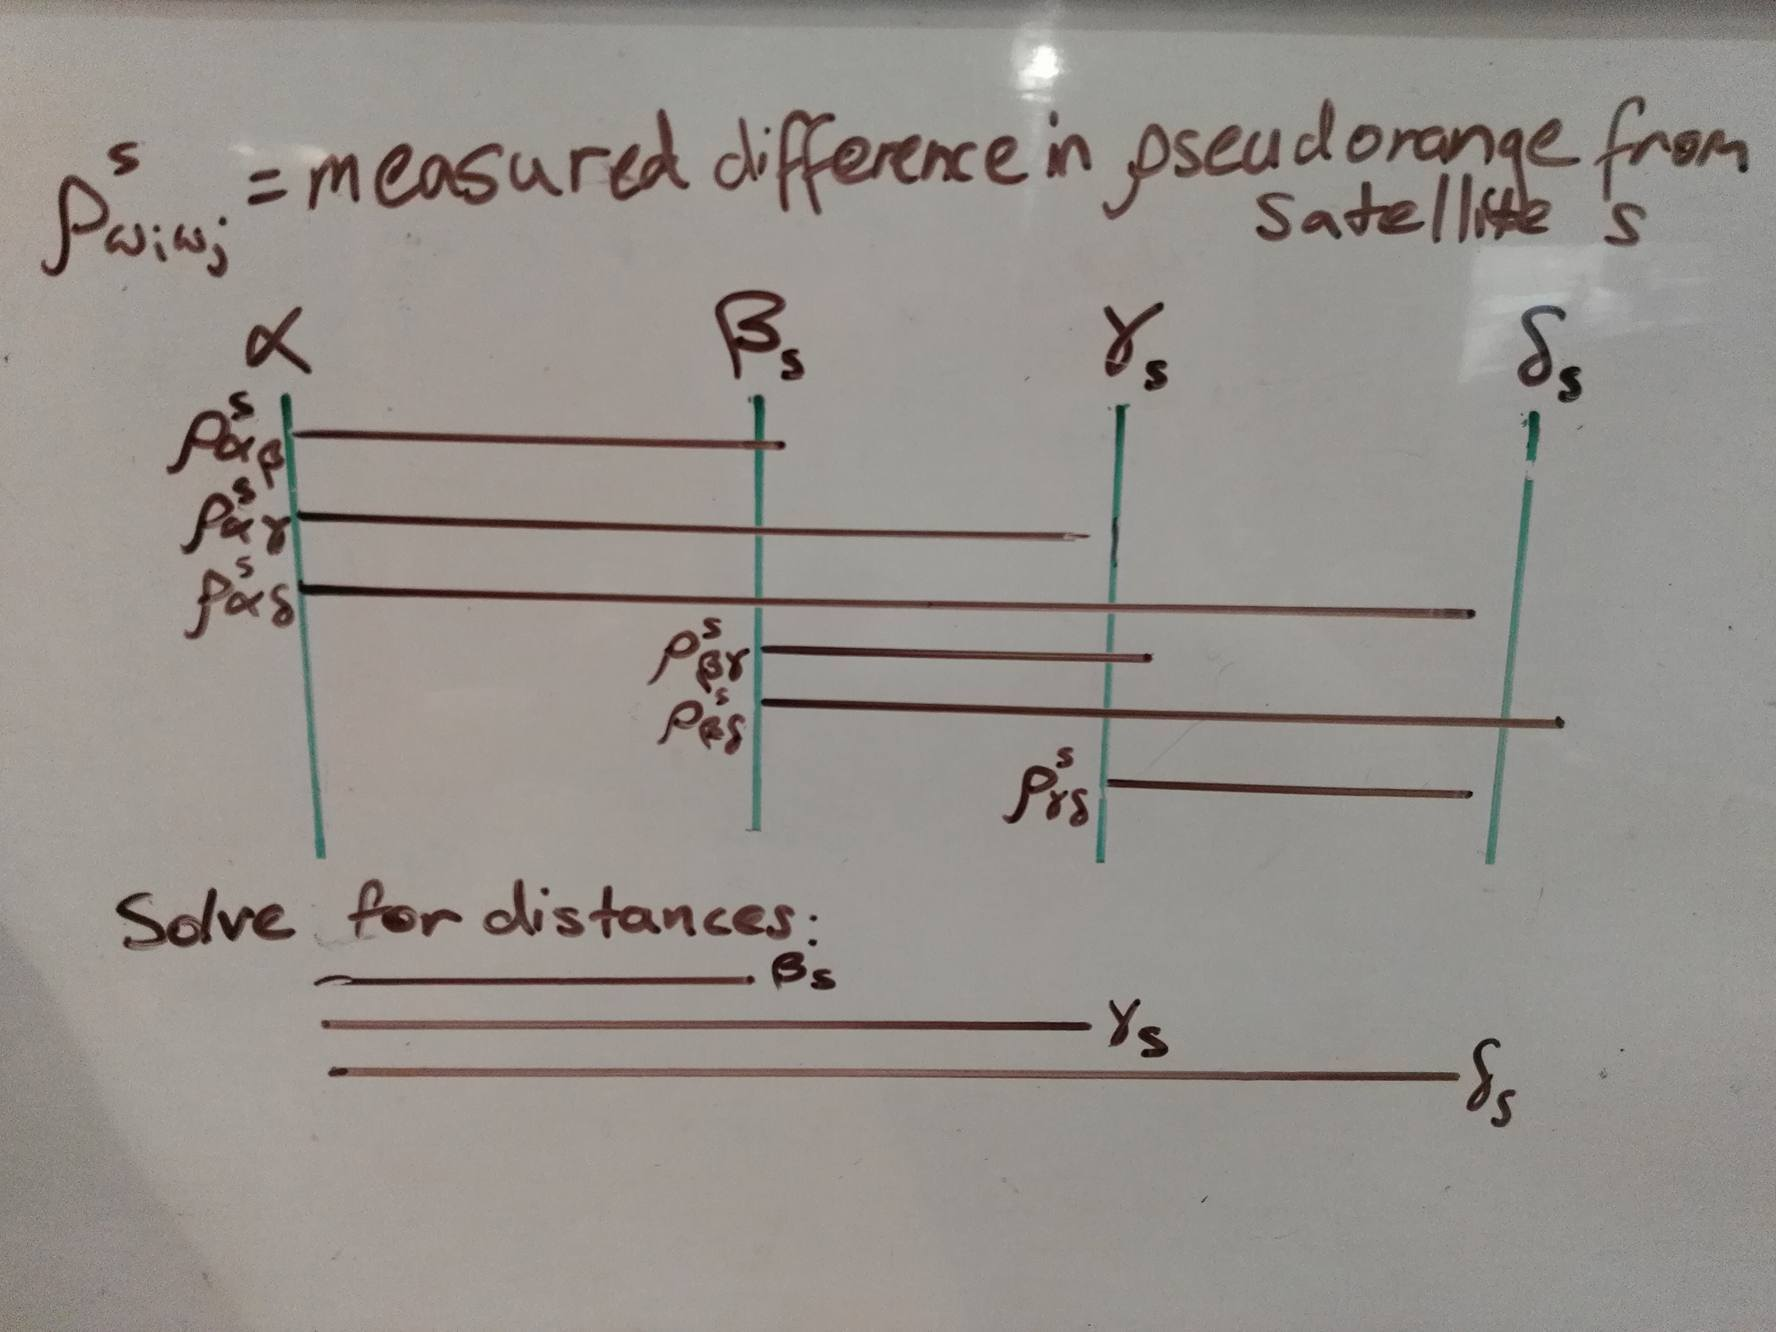
\includegraphics[width=0.7\linewidth]{solve_distances.jpg}
\end{figure}
\begin{eqnarray}
\Phi &=& \begin{bmatrix}
0 & -1 & 0 & ...\\
0 & 0 & -1 & ...\\
... & ... & ... & ... \\
1 & -1 & 0 & ...\\
1 & 0 & -1 & ...\\
\hdotsfor{4} \\
0 & 1 & -1 & ...
\end{bmatrix} \\
%
\Omega_s &=& \begin{bmatrix}
\beta_s \\
\gamma_s\\
\delta_s \\
\vdots
\end{bmatrix} \\
%
\rho_s &=& \begin{bmatrix}
\rho_{\alpha\omega_1}\\
\rho_{\alpha\omega_2}\\
\hdotsfor{1}\\
\rho_{\omega_1\omega_2}\\
\rho_{\omega_1\omega_3}\\
\vdots
\end{bmatrix} 
\end{eqnarray}

\begin{eqnarray}
\Phi\times\Omega_s = \rho_s
\end{eqnarray}
Solve by linear least squares for an overdetermined system by the pseudo inverse matrix
\begin{eqnarray}
\Omega_s = (\Phi^T\Phi)^{-1}\Phi^T\rho_s
\end{eqnarray}

\subsubsection{Point Optimisation}
\paragraph{Create Planes}
Create sets of planes for each receiver $\omega$ from the normal vectors $\hat{\eta_s}$ and the set of distances from the reference point $\alpha$ to receiver $\omega$ along each of the normal vectors denoted $\Omega_\omega$.

The equation of a plane is $Ax+By+Cz+D=0$ where the coefficients [A,B,C] describe the normal vector of the plane and the coefficient D sets the plane in 3D space along the vector. As the normal vector is already calculated for each satellite, only the D coefficient must be solved for each receiver and satellite pair. 
\begin{eqnarray}
P_\omega^s &=& (i\cdot\hat{\eta_s})x + (j\cdot\hat{\eta_s})y + (k\cdot\hat{\eta_s})z + D_\omega^s \label{genplane}\\
P_\omega^s &=& I\cdot H +D_\omega\\
\end{eqnarray}
Where $I = x\hat{\textbf{i}}+y\hat{\textbf{j}}+z\hat{\textbf{k}}$ is the *identity* vector and H is a matrix of normal vectors to each satellite:
\begin{eqnarray}
H = \begin{bmatrix}
\hat{\eta_1} \\
\hat{\eta_2} \\
\vdots\\
\hat{\eta_n}
\end{bmatrix}
\end{eqnarray}
The coefficient D can be calculated by finding a point on the plane $f_\omega^s$, then substituting it into \eqref{genplane} for x,y,z. The point of the plane is calculated by moving along the normal vector by the optimised pseudo distance from the reference point \eqref{Eq:f}.
\begin{eqnarray}
f_\omega^s &=& \Delta_\omega^s\hat{\eta_s} \label{Eq:f}\\
P_\omega^s &=& \hat{\eta_s}\cdot f_\omega^s +D_\omega^s = 0\\
D_\omega^s &=& -\hat{\eta_s}\cdot f_\omega^s\\
D_\omega^s &=& -\Delta_\omega^s ||\hat{\eta_s}|| \\
||\hat{\eta_s}|| &=& 1\\
D_\omega^s &=& -\Delta_\omega^s\\
\Rightarrow P_\omega^s &=& I\cdot H -\Omega_\omega
\end{eqnarray}

\begin{figure}[h]
\centering
\caption{Find position $f_\omega^s$ on the plane}
\label{fig:pointonplane}
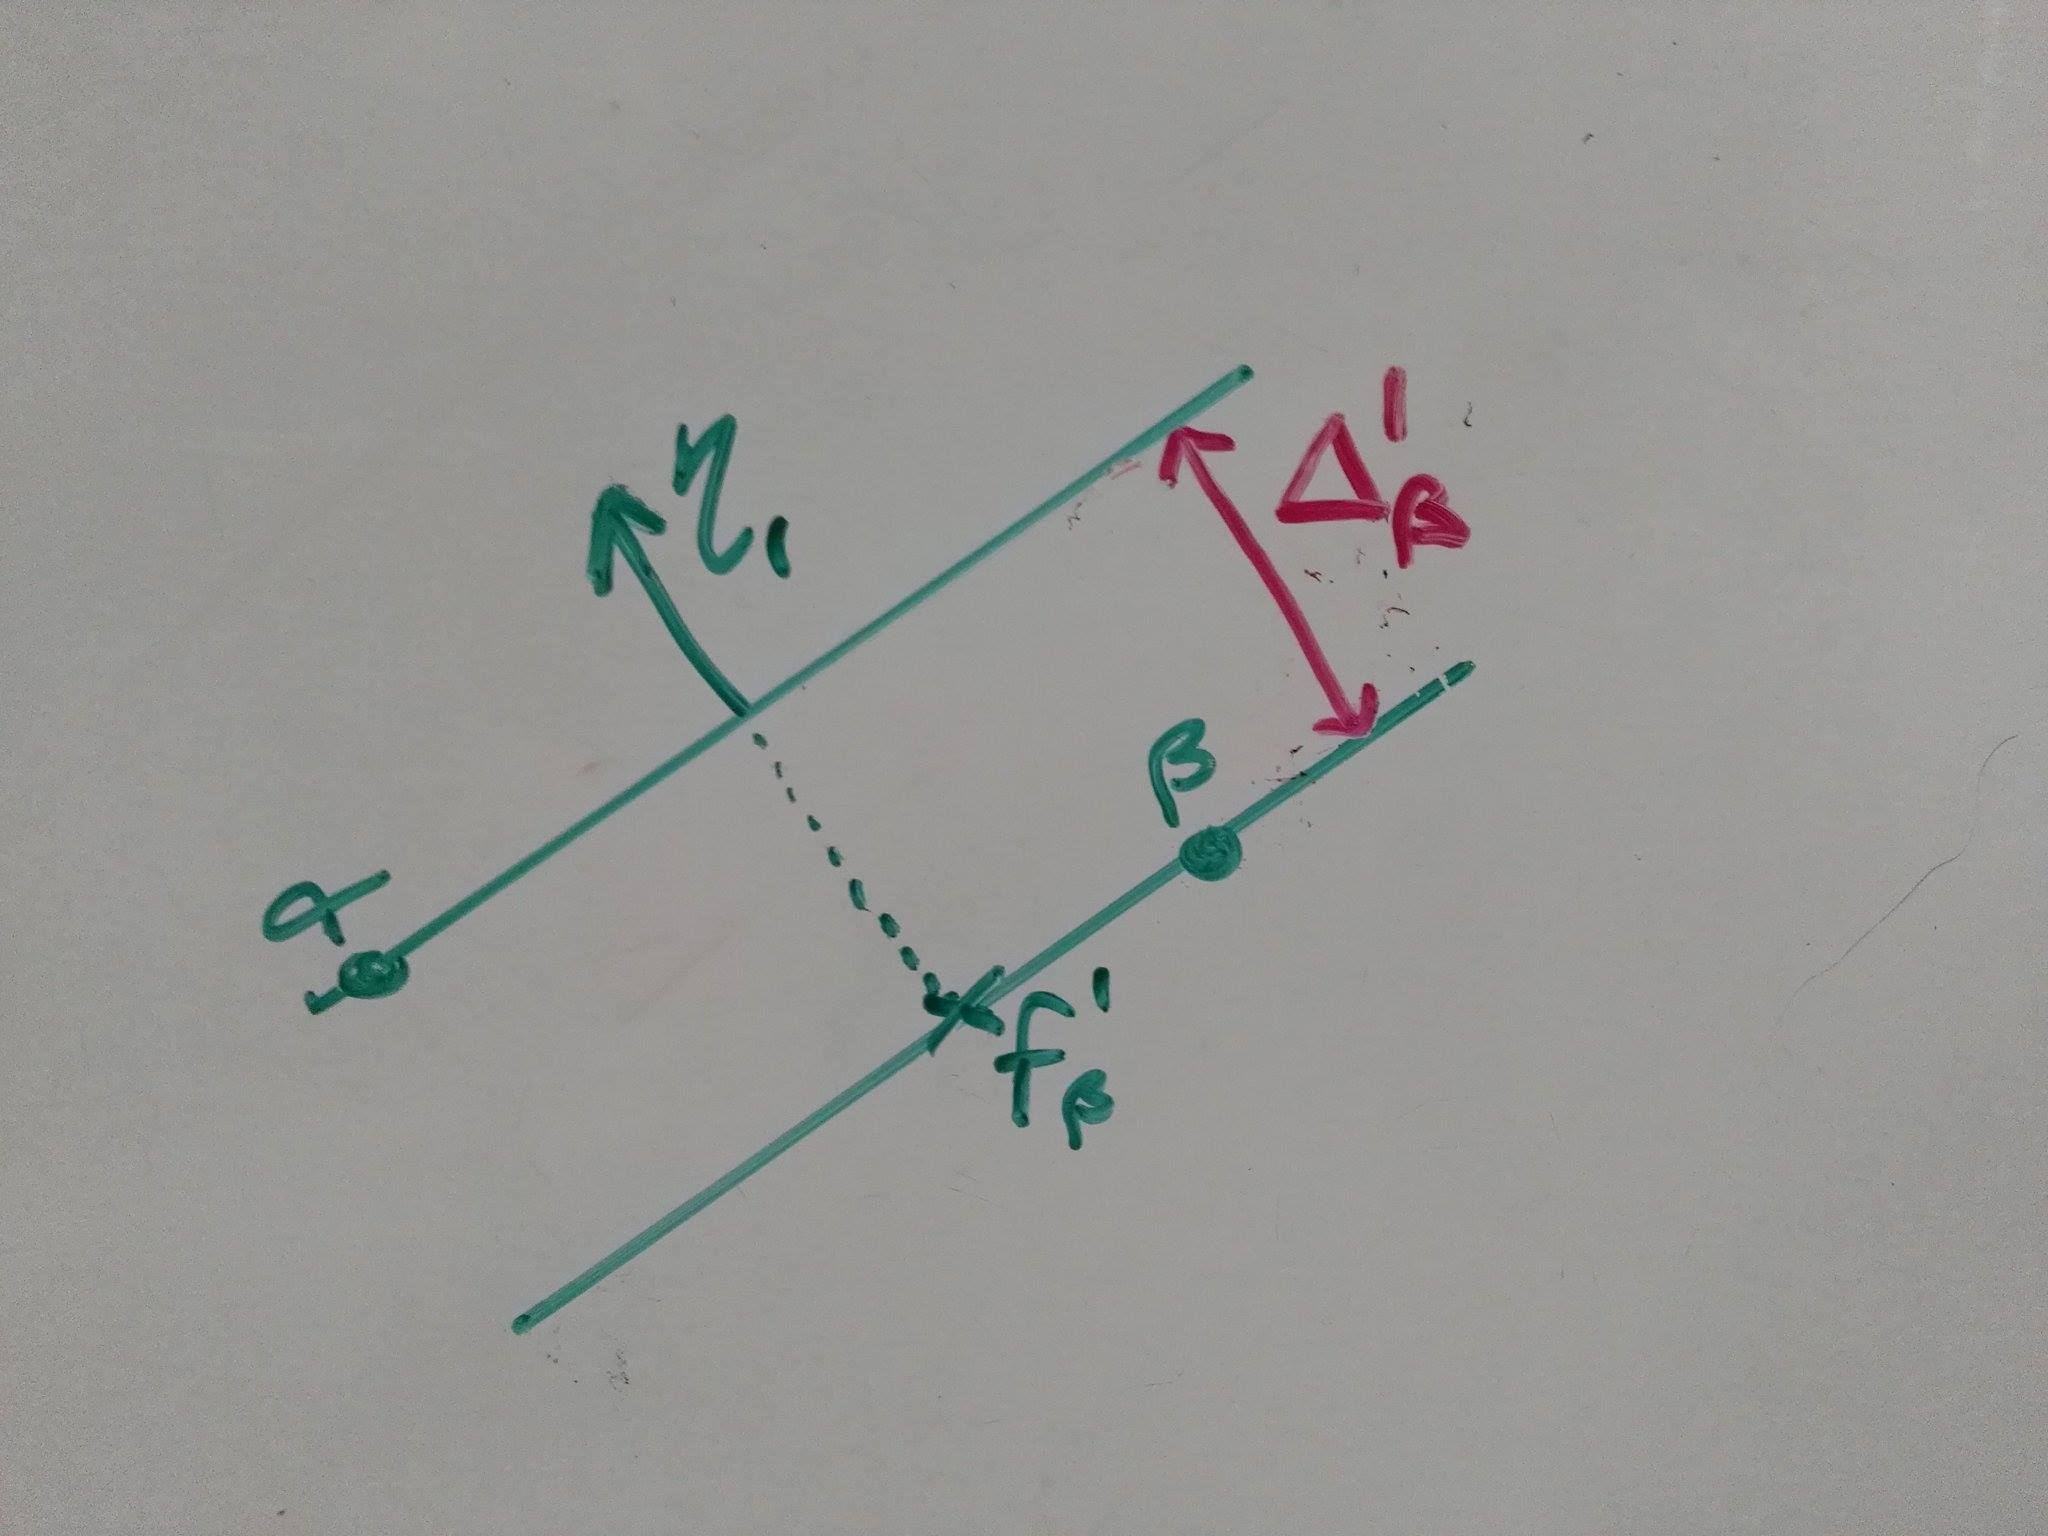
\includegraphics[width=0.7\linewidth]{pointonplane}
\end{figure}






$\Omega_\omega$ is a vector of optimised pseudo-distances from reference $\alpha$ to receiver $\omega$ for all satellites $s\in{1,2...n}$
\begin{eqnarray}
\Omega_\omega = \begin{bmatrix}
\Delta_{\omega}^1 \\
\Delta_{\omega}^2 \\
\vdots\\
\Delta_{\omega}^n \\
\end{bmatrix}
\end{eqnarray}
Where $\Omega_s$ is the vector of optimised pseudo-distances from $\alpha$ to each receiver $\omega\in1,2...m$ for a single satellite s:
\begin{eqnarray}
\Omega_s = \begin{bmatrix}
\Delta_{\omega_1}^s \\
\Delta_{\omega_2}^s \\
\vdots\\
\Delta_{\omega_m}^s \\
\end{bmatrix}
\end{eqnarray}


\paragraph{Solve for Intersection}
As the system of homogeneous linear equations is overdetermined, it can be solved using singular value decomposition to find a point that has the minimum residuals from all of the planes in its set $P_\omega$. Each set of planes for a particular receiver is independent to all other receivers. The vector $X_\omega$ describes the position of receiver $\omega$ in NED coordinates and $\tau_\omega$ describes a final receiver clock bias that alters the displacement of all the planes in the set $P_\omega$ by the same parameter.
\begin{eqnarray}
X_\omega &=& \begin{bmatrix}
x_\omega \\y_\omega \\ z_\omega \\ \tau_\omega
\end{bmatrix}\\
P_\omega X_\omega &=&0 \\
\end{eqnarray}
Minimise error E=eTe where e=PX by imposing a constraint on X. The solution is given by the eigenvector that corresponds to the minimum eigenvalue of ATA. 
 



\section{Method-Simulation}
- what data is it using from receiver? psudorange, time\\

- what errors to include and how to incorporate into the simulation.\\
- how to include the different(asynchronous ) time received for all receivers-> is for the one receiver \\
- how extra receivers affects computational time/ accuracy\\
- how number of sats affect comp time/accuracy\\
- configuration of sats\\
- large multipath affects\\
- no receiver sees the same sat? - does it just output the relative difference between abs values? -> incorrect? just have it fail? not actually implementing, can control the environment\\
- distance of receivers apart\\
- configuration of receivers


- what data received and how to simulate misaligned timing between receivers\\
- what magnitude are the errors and how to simulate them\\
- simulate the errors individually (to see how each type affects the sim - convergence time and accuracy) and/or all errors at once


\subsection{Evaluation} % how to evaluate
- fake gps data\\
- how to simulate noise - what level SNR\\
- to calculate your own GPS location using the normal algorithm? - space 3 \\
- use real GPS locations? (and through time) -space 3\\
- vary number of satellites in view\\
- vary GDOP (good GDOP and bad)\\
- when receivers don't see the exact same satellites \\
- vary number of receivers \\
- simulate a multipath error and how does it account for it or how much error does it introduce\\

How to evaluate?:
- accuracy in relative space\\
- compare to just taking differences in absolute position \\
- between individual receivers and the total error in the whole system\\
- markov? error analysis -> cannot do precision without statistical analysis but isolate errors in x,y,z. how much worse is z than horizontal?\\
- computational time-> how does more receivers/satellites affect the comp time -> what time and space complexity?


\section{Result}



\bibliographystyle{IEEEtran}
\bibliography{bib.bib}
\end{document}